\chapter{Fundamentação Teórica}
\label{ch:fundamentos}

Neste capítulo são abordados conceitos importantes para o entendimento das técnicas que são utilizadas neste trabalho. A Seção \ref{sec:intesification_diversification} apresenta uma introdução sobre diversificação e intensificação, na Seção \ref{sec:evolutionary_algorithms} é introduzido os algoritmos evolutivos, apresentando seus pontos fortes e suas influências para a otimização de problemas complexos. A seguir, na Seção \ref{sec:swarm_intelligence_algorithms} é introduzido os algoritmos de inteligência de enxame e seus pontos positivos na otimização de problemas dinâmicos. Por fim, na Seção \ref{sec:population_diversity} é apresentado a importância da diversidade populacional, mostrando métodos de manutenção e métricas de avaliação.

\section{Intensificação e Diversificação}
\label{sec:intesification_diversification}

A qualidade da otimização de um algoritmo depende do equilíbrio dos componentes de diversificação e intensificação \cite{vcrepinvsek2013exploration}. O equilíbrio adequado permite explorar com mais eficiência o espaço de busca e, consequentemente, obter resultados melhores. A diversificação explora o máximo possível do espaço de busca para identificar diferentes picos de soluções de alta qualidade. Na intensificação ocorre a exploração local, em que se faz a busca mais intensiva em uma área específica. Um algoritmo com rotinas de diversificação em excesso se aproxima de um processo de busca aleatória e um com rotinas de intensificação em excesso leva a uma maior chance de estagnar a busca em um ponto sub-ótimo. 

Esses dois componentes tem ligação direta com a diversidade populacional, de modo que um sistema com muita intensificação gera pouca diversidade. Na Natureza pode-se observar que espécies de animais com grande diversidade tem maiores chances de sobreviver, e para problemas dinâmicos a diversidade é um ponto ainda mais crucial para manter um certo nível de aptidão dos indivíduos durante o processo de otimização.

\section{Algoritmos Evolutivos}
\label{sec:evolutionary_algorithms}
A natureza é uma fonte de inspiração para o desenvolvimento de vários algoritmo, como por exemplo os algoritmos evolutivos. A Computação Evolutiva se inspira no processo da seleção natural e evolução natural. 
Em termos gerais, um algoritmo evolucionário possui alguns componentes básicos para resolução de problemas \cite{parpinelli2011new}:

\begin{enumerate}
\item Representação das possíveis soluções do problema;
\item Um modo de criar uma população inicial (aleatório ou determinístico);
\item Uma função que avalia a qualidade das soluções, ou seja, a aptidão do indivíduo (\textit{Fitness});
\item Um mecanismo de seleção para cruzamento;
\item Operadores evolutivos para criação de novas gerações (como mutação e \textit{crossover});
\item Parâmetros para controle do comportamento do algoritmo, como taxa de cruzamento, taxa de mutação, etc.  
\end{enumerate}

Nas subseções são apresentados os algoritmos do estado da arte no contexto deste trabalho.

\subsection{Algoritmo Genético}
\label{sec:genetic_algorithms}
O Algoritmo Genético (\textit{Genetic Algorithm} - GA) foi um dos primeiros algoritmos bioinspirados a ser proposto durante as décadas de 60 e 70. Ele foi desenvolvido por Holland e seus colaboradores que tem como base a teoria da evolução de Darwin \cite{ga} e é um dos algoritmos mais utilizados na Computação Evolutiva. A seleção natural de Darwin diz que o melhor indivíduo em uma determinada população tem maiores chances de sobreviver e assim passar sua carga genética adiante, tornado a espécie mais apta às condições do ambiente. O GA utiliza essa seleção do indivíduo mais adaptado para direcionar a busca para regiões promissoras no espaço de busca.

A otimização do GA começa com a inicialização da população inicial, sendo de forma aleatória ou determinística, em que cada indivíduo possui um cromossomo, que por sua vez representa uma possível solução para o problema. A partir dessa população inicia-se o primeiro ciclo evolutivo, em que cada indivíduo é avaliado, gerando assim um valor de aptidão (\textit{fitness}) para ser usado na seleção da população. A seleção determina quais indivíduos irão cruzar gerando uma população intermediária, de modo que os mais adaptados possuem uma maior chance de serem selecionados. Os operadores evolutivos de cruzamento e mutação são aplicados na população intermediária, em que o cruzamento tem o papel de intensificar a busca e a mutação o de diversificar a população. A partir deste ciclo o algoritmo se repete até que o critério de parada seja satisfeito.

\subsection{Evolução Diferencial}
\label{sec:diferencial_evolution}
A evolução diferencial (\textit{Diferencial Evolution} - DE) é uma meta-heurística evolucionária para otimização de funções contínuas, proposta por Storn e Price em 1995 \cite{de}. Seu nome se dá pela sua rotina de mutação que acontece por uma operação de subtração (diferenciação). O DE é amplamente estudado e as características que o tornam interessante são: Sua simplicidade, pois é um algoritmo com poucos operadores evolutivos, simples de ser implementado; Seu bom desempenho, tendo uma convergência rápida. O DE se destaca entre vários outros algoritmos evolutivos; e pelo fato de possuir poucos parâmetros, tornando assim sua aplicação mais fácil e intuitiva.

O DE possui, basicamente, uma etapa de inicialização e três etapas em seu ciclo de evolução: mutação, cruzamento e seleção (nessa ordem). O processo evolutivo é iniciado após a inicialização do algoritmo e é finalizado quando um determinado critério de parada for atingido. Primeiramente, o usuário define o tamanho da população ($\lambda$), taxa de chance de \textit{crossover} ($C_r$) e fator de escala ($F$). Existem três tipos de vetores no DE que são: Vetor alvo, que é o vetor pai da geração atual; O vetor doador, que é gerado a partir da mutação; e o vetor \textit{trial}, que é a combinação do vetor alvo com o vetor doador gerado pelo cruzamento. 

Para criar o vetor doador, obtém-se uma amostra de três indivíduos distintos na população. Assim, é criado uma mutação a partir da diferença de dois vetores, multiplicada pelo fator de escala $F$ e somada ao terceiro vetor. A etapa de mutação, responsável pela busca global do algoritmo (diversificação) é o principal fator caracterizante do DE. O $C_r$ controla o cruzamento que é responsável pela intensificação da busca e acontece a partir da recombinação dos vetores alvo e doador. Ao final, a seleção acontece verificando uma melhora no \textit{fitness} do vetor de cruzamento em relação ao alvo, caso não aconteça uma melhora a nova solução é descartada.

\section{Algoritmos de Inteligência de Enxame}
\label{sec:swarm_intelligence_algorithms}
Sistemas baseados em enxames são inspirados pelo comportamento de alguns seres vivos sociais, como formigas, cupins, aves e peixes. A auto-organização e controle descentralizado são características notáveis de sistemas baseados em enxames que, tal como na natureza, levam a um comportamento emergente. Este comportamento é uma propriedade que emerge através de interações locais entre os componentes do sistema e não é possível de ser conseguido por qualquer um dos componentes do sistema atuando isoladamente \cite{garnier2007biological}.

\subsection{Otimização por Enxame de Partículas}
\label{sec:particle_swarm_optimization}
A otimização por enxame de partículas (\textit{Particle Swarm Optimization} - PSO) foi proposta por Kennedy \cite{pso}. O PSO tem como inspiração o comportamento coordenado dos movimentos dos pássaros e cardumes de peixes. Cada partícula é uma solução potencial para o problema, representada por sua velocidade, localização no espaço de busca e uma memória que armazena a sua melhor posição visitada. O movimento de cada partícula depende de sua própria velocidade e da localização das boas soluções encontradas. O equilíbrio entre a intensificação e a diversificação é alcançado no PSO através do comportamento social e o cognitivo, respectivamente.

\subsection{Otimização por Colônia de Bactérias}
\label{sec:biomimicry_bacterial_foraging}
O algoritmo de Otimização por Colônia de Bactérias (\textit{Bacterial Foraging Algorithm} - BFA) foi proposto por Passino \cite{passino2002biomimicry}, inspirado no comportamento social de busca por alimento das bactérias Escherichia Coli. Durante o processo de busca a bactéria se move em pequenos passos enquanto procura alimento. Seu movimento é realizado através de um conjunto de filamentos conhecido como flagelos, que ajudam a bactéria se mover em períodos alternados de natação (\textit{swim}) e tombos (\textit{tumble}). A alternância entre estes dois períodos chama-se quimiotaxia. Cada bactéria representa uma solução para o problema. O ambiente fornece o substrato para as bactérias interagirem e é representado pelo espaço de busca sendo otimizado. Quanto melhor for a região do espaço de busca, melhor será o resultado da função objetivo, e consequentemente, melhor será o substrato para as bactérias.

O BFA é composto por três rotinas principais: quimiotaxia, reprodução e eliminação-dispersão. Na quimiotaxia, uma bactéria com direção aleatória representa um tombo e uma bactéria com a mesma direção do passo anterior indicando uma execução. Na reprodução, a saúde de cada bactéria representa seu valor de \textit{fitness}. Todas as bactérias são classificadas de acordo com seu estado de saúde e apenas a primeira metade da população sobrevive. As bactérias sobreviventes são divididas em dois filhos idênticos, de modo a formar uma nova população. O processo de eliminação-dispersão é responsável por aumentar a diversidade da população. A dispersão ocorre depois de um certo número de etapas de reprodução, quando algumas bactérias são escolhidos de acordo com uma probabilidade predefinida. Tais bactérias são mortas e os novos são gerados aleatoriamente em outra posição dentro do espaço de busca. A intensificação da busca é realizada por ambos os passos de quimiotaxia e de reprodução.

\subsection{Otimização por Colônia de Vaga-Lumes}
\label{sec:firefly_algorithm}
O algoritmo de Otimização por Colônia de Vaga-Lumes (\textit{Firefly Algorithm} - FA) foi proposto por Yang \cite{firefly}. O FA trabalha com 3 regras principais para a otimização, sendo elas:

\begin{itemize}
\item Um vaga-lume será atraído pelo outro não importando o sexo deles;

\item A atratividade entre dois vaga-lumes aumenta em relação a intensidade do brilho e decresce em relação ao aumento da distância entre eles;

\item A proximidade do vaga-lume em relação a uma solução do espaço de busca influencia na intensidade do brilho do mesmo.
\end{itemize}

Cada agente brilha proporcionalmente à qualidade da sua solução que, juntamente com a sua atratividade ($\beta$), ditam o quão forte ela atrai outros membros do enxame. Dois outros parâmetros definidos pelo usuário são o valor máximo de atração ($\beta_i$) e do coeficiente de absorção ($\Upsilon$) que determina a variação de atratividade com o aumento da distância da comunicação dos vaga-lumes. A variável
de intensidade da luz $\beta_i$ de cada vaga-lume, mantém o balanço entre a intensificação e diversificação da busca.

\subsection{Otimização por Colônia de Morcegos}
\label{sec:bat_algorithm}
O algoritmo de Otimização por Colônia de Morcegos foi apresentado pela primeira vez por Yang \cite{bat}. O algoritmo é inspirado no processo de eco-localização dos morcegos utilizado durante o seu voo para detectar presas e evitar obstáculos. além disso é utilizada uma rotina de voo aleatório para movimentação no espaço de busca, atualizando suas posições e suas velocidades. Outros parâmetros são: o fator de decaimento de sonoridade ($\alpha$) que atua em um papel semelhante a temperatura do \textit{simulated annealing}, e o fator de aumento de pulso ($\gamma$) que regula a frequência de pulso. A atualização da taxa de pulso ($R_i$) e sonoridade ($A_i$) equilibra o comportamento intensificação e diversificação de cada morcego, respectivamente. De acordo com a diminuição da sonoridade a taxa de pulso vai aumentando para melhorar a acurácia do ataque. 

\subsection{Algoritmo de Busca por Cardume de Peixes}
\label{sec:fish_school_search}
O algoritmo de Busca por Cardume de Peixes (\textit{Fish School Search} - FSS) foi proposto por Carmelo \cite{carmelo2008novel} inspirado pela busca de fontes de alimento por um cardume de peixes. O processo de pesquisa do FSS é feito por uma população de indivíduos, com memória limitada, representando o peixe. O ambiente de busca é representado pelo mar em que os peixes se encontram, onde eles podem se movimentar para tentar melhorar sua solução. A densidade de comida representa a qualidade da solução, de forma que em um problema de maximização a densidade de comida é diretamente proporcional a qualidade do resultado. A densidade de comida de um local influencia o peixe através do peso, de forma que uma melhora continua da solução apresenta um peixe mais pesado.

\subsubsection{Operadores Evolutivos}
\label{sec:evolutionary_operators}
A versão do algoritmo estudada é versão canônica, que possui 4 operadores com suas funções bem definidas e são separados em duas classes \cite{bastos2009influence}: Alimentação (OA) e Movimentação. Para a movimentação tem-se as seguintes classificações: Operador de Movimento Individual (OMI); Operador de Movimentação Coletiva Instintiva (OMCI); e Operador de Movimentação Coletiva Volátil (OMCV).

Como representado na na Figura \ref{fig:pseudo_code} o processo evolutivo do FSS acontece: primeiramente a população inicial é gerada aleatoriamente, depois ela é avaliada. Assim, o ciclo evolutivo começa. O cliclo principal é dividido em 3 outros ciclos menores, em que cada um deles representa um operador de movimento. No primeiro ciclo é feita a avaliação da nova geração, depois é calculado o OMI e os peixes que realizaram esse movimento são marcados e tem seus pesos atualizados, por fim outra avaliação da população é feita. No segundo ciclo é calculado o OMCI e aplicado em todos os peixes do cardume, mesmo os que não realizaram o movimento individual. No terceiro ciclo é feito o movimento volátil, em que, se a população em geral sofreu uma melhora no peso (melhora nos resultados encontrados), ela contrai, e se a população sofreu uma piora no peso, ela dilata. Por fim são atualizados os pesos e as variáveis de $step_{ind}$ e $step_{vol}$ (variáveis que determinam a intensidade que os movimentos irão afetar o cardume, elas diminuem linearmente ao decorrer do processo evolutivo).

\begin{figure}[!htb]
	\caption{Diagrama de blocos do FSS}
	\centering
	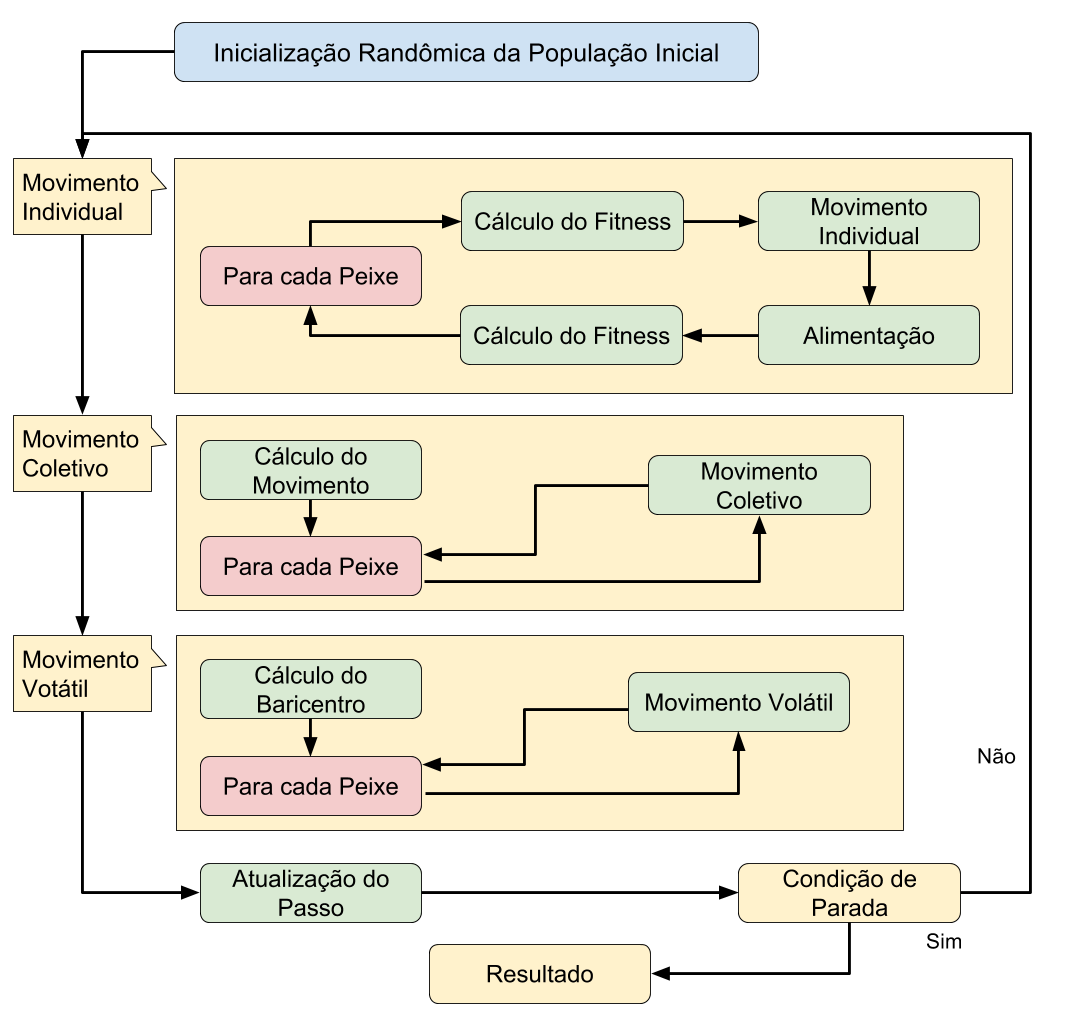
\includegraphics[scale=0.4]{images/diagrama_blocos.png}
	\label{fig:pseudo_code}{\\Fonte: Produção do próprio autor.}
\end{figure}

\noindent \textbf{Operador de Movimento Individual - OMI}

O OMI representa o movimento de cada um dos peixes individualmente, sem a influência do cardume. A próxima posição (candidata) é determinada pela geração de um número aleatório de uma distribuição normal e esse número é atribuído a uma das posições vizinhas do indivíduo. Após, o número é multiplicado por uma variável chama de $Step_{ind}$, que é a percentagem da amplitude do espaço de busca, essa variável decresce linearmente durante cada iteração, como mostrado na Equação \ref{eq:individual_moviment}.

\begin{equation}
\label{eq:individual_moviment}
\begin{split}
& n_i(t) = x_i(t) + N(-1,1).Step_{ind} \\
& \Delta f = f(\vec{n}) - f(\vec{x}) \\
& \Delta \vec{x} = \vec{n} - \vec{x} \\
& Step_{ind}(t+1) = Step_{ind}(t) - \frac{Step_{indInicial} - Step_{indFinal}}{iteracoes};
\end{split}
\end{equation}

\noindent Em que $n_i$ é a nova posição candidata, $x_i$ é a posição atual, $\Delta f$ é a variação do \textit{fitness}, o $\Delta x$ a variação do movimento e o $N(-1,1)$ é uma distribuição normal aleatória. A nova posição é efetivamente atualizada, somente se, ela for melhor que a posição anterior do indivíduo. Sendo assim, pode-se observar que esse operador tem influência na busca global feita por cada indivíduo.

\noindent \textbf{Operador de Alimentação - OA}

Quando são gerados, os peixes possuem o mesmo peso e ao longo da busca esse peso é alterado de acordo com o melhoramento da solução, ou seja, caso a solução melhore o peso aumenta. O peso de cada peixe representa o quão bem o indivíduo está na busca da solução. O cálculo do peso tem influência da população, utilizando maior variação de \textit{fitness} encontrada entre todos os indivíduos como $\max{\Delta f}$, sendo a diferença entre o melhor e o pior indivíduos, mostrado na Equação \ref{eq:food_operator}.

\begin{equation}
\label{eq:food_operator}
W_i(t+1) = W_i(t) + \frac{\Delta f_i}{\max{\Delta f}}
\end{equation}

\noindent \textbf{Operador de Movimentação Coletiva Instintiva - OMCI}

Somente os indivíduos que realizaram o OMI, ou seja, $\Delta x$ tem que ser diferente de zero, terão influência no cálculo do movimento coletivo. Após o cálculo do movimento coletivo $\vec{I}(t)$, em que é avaliado a variação do \textit{fitness} dos peixes em relação a do cardume, todos os indivíduos são atualizados, mesmo os que não realizaram o movimento individual. Como mostrado na Equação \ref{eq:coletive_instintive}. Esse operador coletivo instintivo tem como contribuição a busca local fazendo com que a população inteira se direcione para um espaço de busca possivelmente melhor, simulando assim, o efeito de um cardume de peixes.Na Figura \ref{fig:coletive_moviment} pode-se observar que todo o cardume se movimenta na mesma direção dos melhores indivíduos, que são os círculos maiores.

\begin{equation}
\label{eq:coletive_instintive}
\begin{split}
& \vec{I}(t) = \frac{\sum_{i=1}^{n} \Delta \vec{x}_i \Delta f_i}{\sum_{i=1}^{n} \Delta f_i} \\
& \vec{x}_i (t+1) = \vec{x}_i (t) + \vec{I}(t)
\end{split}
\end{equation}

\begin{figure}[!htb]
	\caption{Representação gráfica da influência do Movimento Coletivo Instintivo na população}
	\centering
	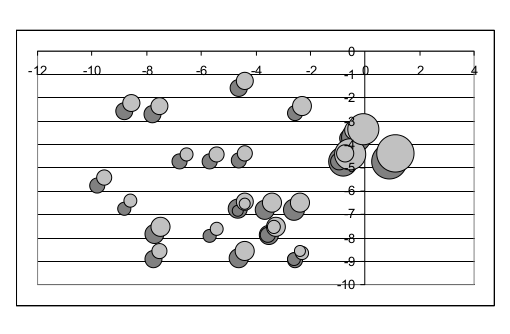
\includegraphics[scale=0.5]{images/movimento_coletivo.png}
	\label{fig:coletive_moviment}{\\Fonte: \citeonline{c2009influence}.}
\end{figure}

\noindent \textbf{Operador de Movimentação Volátil Coletiva}

Este movimento é baseado na melhora em geral da população, que é representada através do peso médio da população. Quando tem-se uma melhora nas soluções ocorre a contração da população em relação ao baricentro dos indivíduos, caso contrário, ocorre a dilatação. O cálculo do baricentro $\vec{B}(t)$ é feito com base na posição de cada indivíduo e o peso de cada um deles. Todos os indivíduos da população são afetados pela contração $\vec{x}_{contract}$ ou dilatação $\vec{x}_{dilat}$, de forma que a busca pode ficar mais focada em um ponto, ou expandida para buscar mais resultados, como mostrado na Equação \ref{eq:volitive_instintive}. 

Na Figura \ref{fig:volitute_moviment} pode-se observar uma contração que mostra um intensificação do espaço de busca. Esse operador tem como maior contribuição tanto a manutenção da variabilidade genética, de forma que ajuda a busca a não ficar presa em um ótimo local, quanto a intensificação da mesma, pois quando acontece uma contração a busca naquele local fica mais concentrada.

\begin{equation}
\label{eq:volitive_instintive}
\begin{split}
& \vec{B}(t) = \frac{\sum_{i=1}^{n} \vec{x}_i  w_i(t)}{\sum_{i=1}^{n} w_i(t)} \\
& \vec{x}_{contract}(t+1) = \vec{x}_{contract}(t) - step_{vol}N(0,1) \frac{\vec{x}(t)-\vec{B}(t)} {\textit{distance}(\vec{x}(t),\vec{B}(t)))}
\end{split}
\end{equation}

\begin{figure}[!htb]
	\caption{Representação gráfica da influência do Movimento Coletivo Instintivo de uma contração}
	\centering
	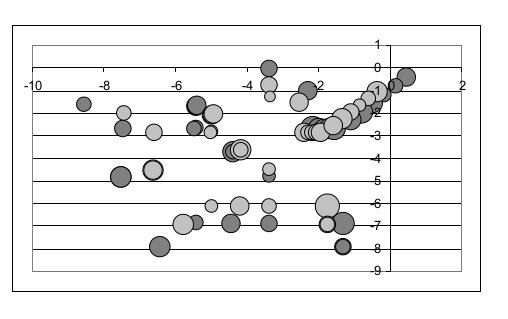
\includegraphics[scale=0.5]{images/movimento_volatil.png}
	\label{fig:volitute_moviment}{\\Fonte: \citeonline{c2009influence}.}
\end{figure}

\section{Diversidade Populacional}
\label{sec:population_diversity}
Uma população com diversidade pode ser capaz de lidar com funções multimodais e explorar simultaneamente diferentes picos na superfície da função objetivo, como também melhorar a exploração global e ajudar a encontrar vários ótimos globais e locais.

Em problemas dinâmicos uma boa diversidade populacional ajuda o sistema a manter um nível satisfatório de \textit{fitness} durante todo o processo de otimização. Ajuda também o sistema a se adaptar as mudanças no ambiente, de forma que, ao perceber essa mudança os indivíduos mais afastados dos pontos ótimo podem encontrar diferentes soluções que podem se tornar novos pontos ótimos.

Além disso, muitos dos problemas dinâmicos possuem mais de um ponto ótimo e algumas estratégias de manutenção da diversidade populacional, mostradas na Seção \ref{sec:maintain_diversity} ajudam a encontrar vários pontos ao mesmo tempo.

\subsection{Manutenção}
\label{sec:maintain_diversity}
As principais estratégias encontradas na literatura são o \textit{fitness sharing, clearing, crowding, deterministic crowding} e \textit{probabilistic crowding}.

Compartilhamento (\textit{Sharing}): Foi introduzido por Goldberg e Richardson \cite{sharing}, com a intenção de localizar múltiplos picos simultaneamente. A ideia básica é punir indivíduos que ocupam as mesmas regiões no espaço de busca por escala a aptidão de cada indivíduo de acordo com o número de indivíduos na vizinhança. Assim, penalizando indivíduos que se aglomeram em conjunto, o regime de partilha impede a convergência para um único pico. O \textit{fitness sharing} de um indivíduo $i$ é definido pela Equação \ref{eq:sharing}. Onde $n$ é o número de indivíduos da população, $\sigma_{share}$ indica o limiar de dissimilaridade e $d_j^i$ é a medida de distância entre o indivíduo $i$ e $j$.

\begin{equation}
\label{eq:sharing}
\begin{split}
& f_{share}^i = \frac{f_i}{\sum_{j=0}^{n} sharing_j^i} \\
& sharing_j^i =
	\begin{cases}
	1 - (d_j^i/\sigma_{share})^2 	& \quad \text{Se } d_j^i < \sigma_{share}\\
	0 							& \quad \text{Se não}\\
	\end{cases} 
\end{split}
\end{equation}

Compensação (\textit{clearing}): é um método similar ao Compartilhamento, porém é baseado no conceito de recursos limitados no ambiente \cite{clearing}. Ao invés de compartilhar recursos entre todos os indivíduos de uma subpopulação, o método de compensação atribui o \textit{fitness} apenas para os melhores indivíduos da subpopulação. Assim, o \textit{clearing} preserva o \textit{fitness} dos $k$ melhores indivíduos do nicho e redefine o \textit{fitness} dos outros que pertencem à mesma subpopulação. Como no método de \textit{sharing}, indivíduos pertencem ao mesmo nicho se sua distância no espaço de busca for menor que um limiar de dissimilaridade $\sigma_s$ (raio de \textit{clearing}). O \textit{clearing} pode ser combinado com estratégias de elitismo para preservar as melhores soluções dos nichos durante gerações.

Aglomeração (\textit{Crowding}): O método de \textit{Crowding} foi proposto por De Jong \cite{crowding}. Este método de nichos de espécies compara um descendente com alguns indivíduos escolhidos aleatoriamente da população atual. O indivíduo mais semelhante será substituído se o descendente oferecer melhor valor de \textit{fitness}. O fator de aglomeração (parâmetro $CF$) é definido como uma pequena parcela da população, o qual é utilizado para controlar o tamanho da amostra. Nesse método existe a possibilidade de se sobrescrever um mesmo indivíduo várias vezes, esse fato se chama erro de substituição que é a principal desvantagem do \textit{Crowding}, além disso, o \textit{Crowding} é propenso a aglomeração de indivíduos ao redor das picos de soluções ótimas.

Aglomeramento Deterministico (\textit{Deterministic Crowding}): Para aliviar o problema de erro de substituição, foi introduzido uma melhoria na aglomeração original, que não utiliza o parâmetro do fator de aglomeração. Este método foi chamado aglomeração determinista \cite{deterministic_crowding}. Essa abordagem minimiza o erro de substituição significativamente e restaura a pressão seletiva. No entanto, este método também tem uma desvantagem em que aumenta a perda de nichos devido ao uso de seleção por torneio entre indivíduos semelhantes.

Aglomeramento Probabilístico (\textit{Probabilistic Crowding}): Para superar o problema da falta ótimos locais foi criado o método de aglomeração probabilística \cite{probabilisti_crowding}. A regra de substituição probabilística é usada para manter uma elevada diversidade na população que substitui indivíduos de menor \textit{fitness} por indivíduos de \textit{fitness} mais elevados de acordo com a sua proporção de \textit{fitness}. O principal problema deste processo é que ele tem uma taxa de convergência muito lenta e baixa capacidade de pesquisa.

Lacuna de Geração (\textit{Generation Gap}): Neste modelo apenas uma parte da população (\textit{generation gap}) se reproduz e morre em cada geração. Deste modo o filho substitui o indivíduo mais similar retirado de uma subpopulação aleatória de tamanho $CF$ (\textit{crowding factor}) da população total. 

\subsection{Métricas}
\label{sec:evaluete_diversity}

Para poder avaliar o estado da diversidade de uma população são utilizados dois tipos de medidas de diversidade: A medida de diversidade fenotípica (MDF) e genotípica (MDG). A MDF mede a diversidade de \textit{fitness} das soluções, ou seja, a diversidade de diferentes qualidades de soluções. Já a MDG mensura a diversidade genética das soluções, avaliando o conjunto de variáveis (genes) que influenciam na função objetivo.

A MDF é apresentada na equação \ref{eq:fenotype}, em que variável $VMD$ é um fator de normalização que corresponde a medida de diversidade de uma população virtual com os valores de \textit{fitness} distribuídos de maneira uniforme com uma distância predeterminada. Onde $f_{worst}$ representa o pior \textit{fitness} e o $f_{best}$ o melhor \textit{fitness} e $N$ o tamanho da população \cite{phenotypic}. Quando o tamanho da população ou a faixa de \textit{fitness} absoluto são modificados é necessário recalcular o $VMD$. É importante ressaltar que para calcular a MDF é preciso que os valores de \textit{fitness} estejam ordenados.

\begin{equation}
\label{eq:fenotype}
\begin{split}
& MDF = \frac{\sum_{i=0}^{n-1} \ln(1 + |f_i - f_{i+1}|)}{VMD} \\
& VMD = \sum_{i=0}^{n-1} \ln(1 + |f_i - f_{i+1}|)
\end{split}
\end{equation}

A MDG  proposta por Corriveau \cite{genotypic}. Esta medida foi desenvolvida com base na MDF, sendo indicada para variáveis contínuas. A medida é apresentada na Equação \ref{eq:genotypic}, onde $D$ é a quantidade de dimensões da solução, $N$ o tamanho da população e $x$ a solução candidata. A variável
$NMDF$ é o fator de normalização que corresponde ao valor máximo de diversidade conhecida até o momento. O valor 1 obtido da medida corresponde a diversidade genotípica máxima enquanto o valor 0 corresponde a convergência da população de soluções.

\begin{equation}
\label{eq:genotypic}
MDG = \frac{\sum_{i=0}^{n-1} \ln \left(1 + \min_{j \in [i_1,N]} \frac{1}{D} \sqrt{ \sum\limits_{k=1}^{D} (x_{i,k} - x_{j,k})^2}\right)}{NMDF}
\end{equation}

\section{Aplicação do AG em ambientes dinâmicos}
\label{sec:ag_behaviour}

Um trabalho que pode ser citado em relação a avaliação de algoritmos em ambientes dinâmicos é o trabalho de \cite{rand2005measurements}, em que é feita uma análise do comportamento do AG em um ambientes dinâmicos discreto. Mesmo sendo um trabalho que é aplicado em uma classe de problemas diferente da abordada por este trabalho, ele mostra que na maioria dos trabalhos que analisam um algoritmo somente avaliam o desempenho, ou seja, o quão perto do melhor resultado chegou. São analisados quatro fatores principais para determinar a eficiência do AG em ambientes dinâmicos, sendo eles:

\begin{enumerate}
	\item Desempenho: Para entender o desempenho do algoritmo existem duas vertentes, sendo uma a avaliação do melhor indivíduo da população para cada iteração do AG, e a outra é avaliar a média da população em para cada uma das iterações. Para a aplicar AG no SL-HDF é usado a melhor solução antes da primeira alteração como média inicial.
	
	\item Satisfabilidade: É a medida da habilidade do sistema de manter um certo nível de \textit{fitness} no decorrer da otimização e não deixar esse nível cair abaixo de um determinado limite. Esta medida não necessariamente representa o quão rápido (menos interações necessárias) o sistema chega em uma nova ótima solução, e sim se ele consegue manter um nível de \textit{fitness} da população.
	
	\item Robustez: É a medida de como o sistema reage a uma alteração, de forma que ao sofrer uma alteração o \textit{fitness} não pode ter uma queda muito brusca. A medida de robustez usada neste trabalho foi a média do \textit{fitness} no estado atual do ambiente sobre a média do \textit{fitness} no estado anterior do sistema, para uma alteração perceptível.
	
	\item Diversidade: É a medida que representa a variação do genoma da população, de forma que uma população que possui uma alta diversidade tem maiores chances de encontrar novas solução e assim se adaptar melhor a uma mudança do ambiente. Existem várias técnicas estudadas para manter a diversidade da população durante o processo evolutivo, e para medir a diferença genotípica é usado a distância de \textit{Hamming}.
\end{enumerate}

Na aplicação do AG pode-se notar que a performance do algoritmo no ambiente dinâmico é superior sua aplicação em ambientes estáticos quando há um grande número de iterações. Inicialmente o ambiente dinâmico perde para o estático mas a partir da metade do processo evolutivo o dinâmico gera um \textit{fitness} maior no melhor indivíduo e na média da população.

A análise da satisfabilidade mostra o nível do \textit{fitness} durante o processo evolutivo, e com ele pode-se notar que mesmo em relação a uma aplicação em um ambiente estático, o nível de \textit{fitness} pode ser mantido acima de um limiar.

Na análise de robustez pode-se notar que a cada mudança no ambiente existe uma queda na média do \textit{fitness}, porém o sistema se recupera rapidamente, e a cada nova mudança e queda do \textit{fitness} diminui.

A diversidade do sistema teve um comportamento inesperado, pois inicialmente achava-se que o sistema iria perder a diversidade até uma mudança ocorrer e depois a diversidade iria aumentar, porém aconteceu exatamente o contrário, tendo que após uma mudança a diversidade diminui e vai aumentando até identificar uma nova mudança.